%=========================================================
%------------Cabeçalho e rodapé 
%=========================================================
\pagestyle{headandfoot}%{head}%empty
\firstpageheader{}{}{}
\runningheader{\disciplina}{}{\avaliacao}
\runningheadrule
\firstpagefooter{\professor}{}{Pag. \thepage\ de \numpages}
\runningfooter{\professor}{}{Pag. \thepage\ de \numpages}
\runningfootrule
%===============================================================
%INFORMAÇÕES SOBRE A AVALIAÇÃO
\nomeInst{Instituto Federal do Ceará}
\logoInst{
\includegraphics[scale=0.4]{Figs/ifbajequie.jpg}}
\Campus{Tauá} %COMENTE ESTA LINHA SE FOR ENSINO FUNDAMENTAL OU MÉDIO
\nomeCurso{Análise e Desenvolvimento de Sistemas} %Se não for curso superior, basta comentar esta linha
\nomeDisciplina{Ciência de Dados}
\DataProva{}
\Turma{}
\Semestre{5º}
\nomeProfessor{Prof. Reginaldo Fernandes}
\Aluno{}
\matriculaAluno{}
%Caso não queira imagem de fundo, basta comentar a linha abaixo
%\ImagemFundo{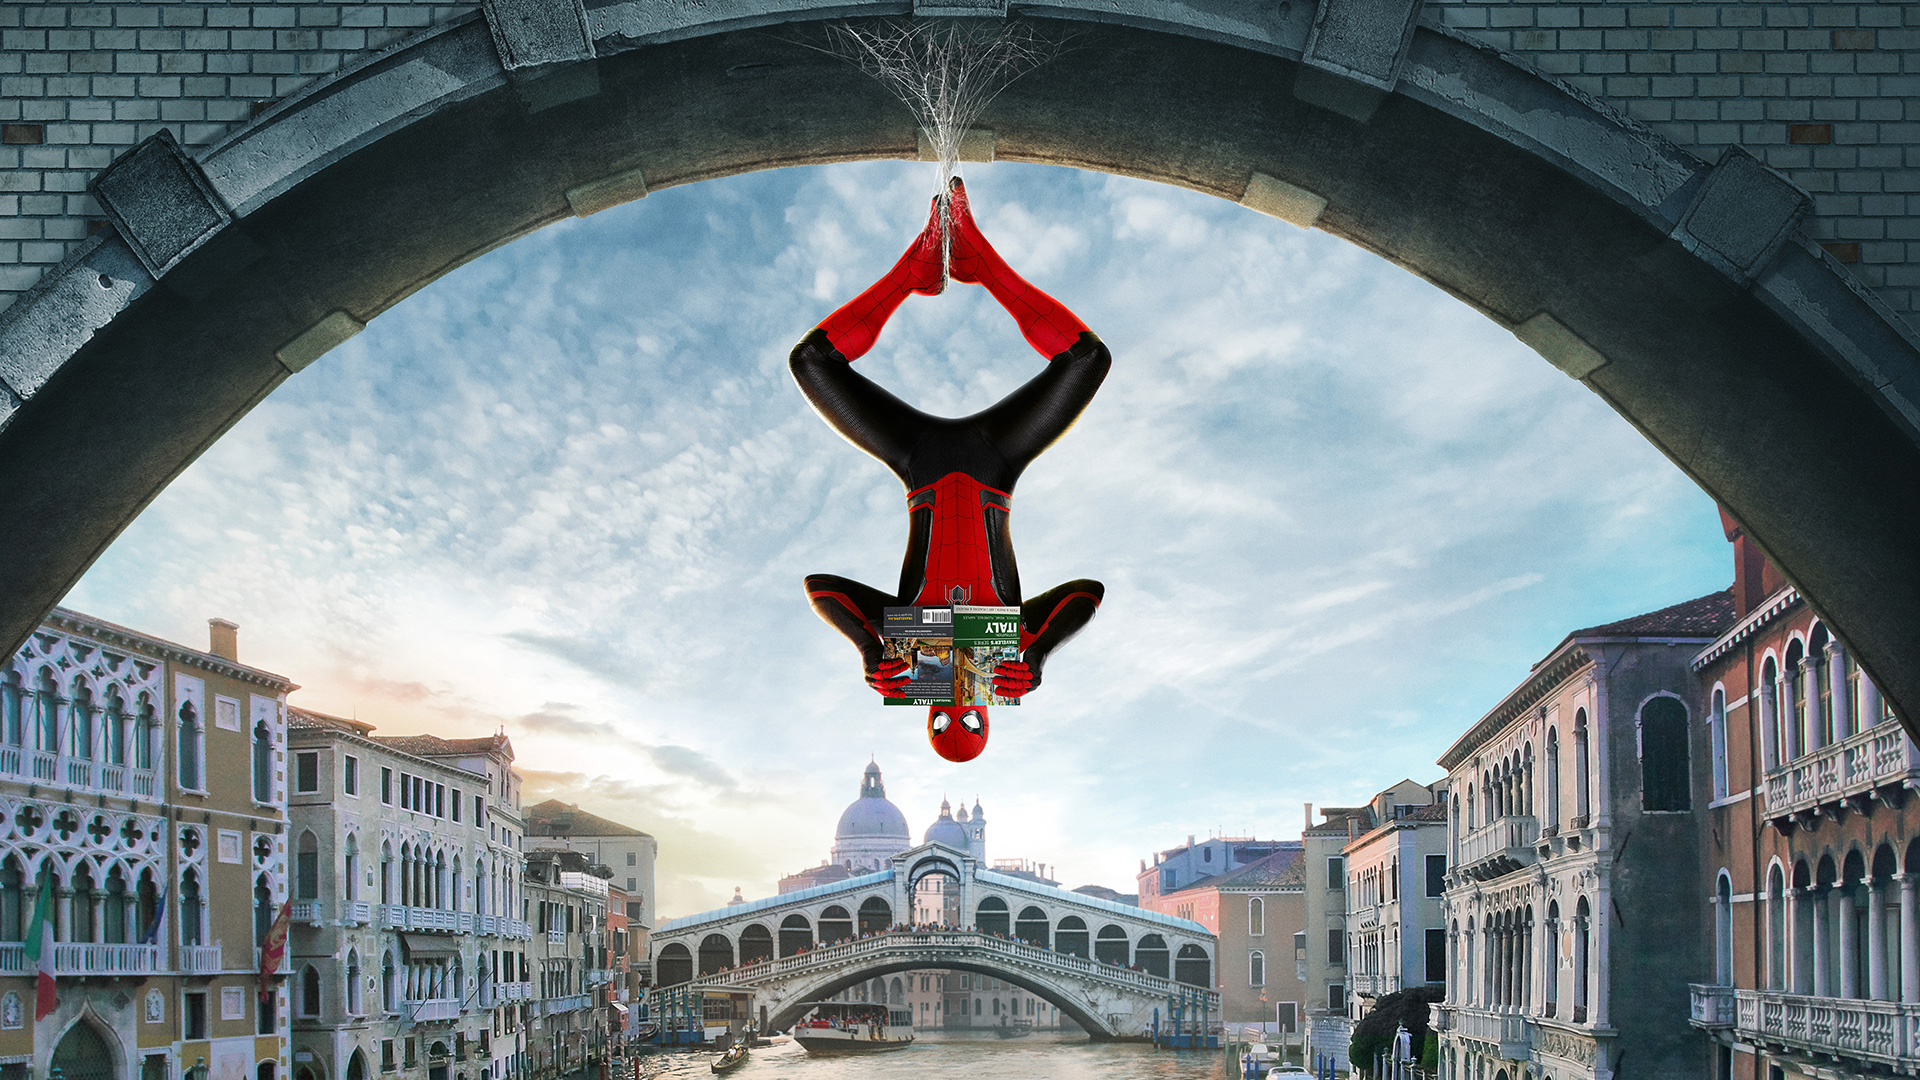
\includegraphics[height=\paperheight]{Figs/Fundo/aranha2.jpeg}}
%===============================================================

%INSTRUÇÕES PARA A AVALIAÇÃO, deixe em branco as que não quiser colocar
\instum{Sua avaliação consta de \numquestions \ questões, somando \numpoints \  pontos. \textbf{É proibido utilizar consultas.}} 
\instdois{\textbf{A posse de celular durante a avaliação será entendida como cola, independentemente do uso.}}
\insttres{}
\instquatro{}
\instcinco{}
\instseis{}